% ============================================
% VCP: Single-Stage Cosine Classifier and Prototype Learning
%   for Few-Shot Object Detection
% IEEE Conference Paper — 4-page version
% ============================================

\documentclass[conference]{IEEEtran}
\IEEEoverridecommandlockouts

\usepackage{cite}
\usepackage{amsmath,amssymb,amsfonts}
\usepackage{graphicx}
\usepackage{booktabs}
\usepackage{multirow}
\usepackage{hyperref}
\usepackage{stfloats}

\begin{document}

\title{VCP: Single-Stage Cosine Classifier and Prototype Learning for Few-Shot Object Detection}

\author{\IEEEauthorblockN{Xiang Fei}
\IEEEauthorblockA{\textit{School of Engineering, Qufu Normal University} \\
Rizhao, Shandong 276826, China \\
felix.fei@qfnu.edu.cn}
}

\maketitle

\begin{abstract}
Few-shot object detection (FSOD) methods are almost exclusively built upon the two-stage Faster R-CNN, while YOLO-series single-stage detectors---dominant in industrial deployment---lack systematic FSOD investigation. We present VCP (Visual-Cosine-Prototype), a single-stage FSOD framework combining YOLO11s with a cosine classifier and prototype learning under the TFA protocol. On PASCAL VOC, VCP achieves 72.2\% mAP50 (3-split mean) at 10-shot with only 9.5M parameters ($\sim$1/6 of competing methods). However, the same approach underperforms fine-tuning on MS COCO. Through systematic Precision-Recall decomposition across 24 comparison groups, we reveal that the cosine classifier acts as a \textit{Recall Booster}---consistently pushing the operating point toward higher recall and lower precision. We formulate the P-R Tradeoff Hypothesis: the net benefit depends on the product of baseline recall headroom and the dataset-specific P-R tradeoff ratio, explaining the VOC-COCO divergence. We further explore Florence-2 VLM semantic prototypes as auxiliary priors (+0.5 pp at 10-shot). VCP runs at 54.4 FPS, 4--5$\times$ faster than two-stage FSOD methods with zero VLM inference overhead.
\end{abstract}

\begin{IEEEkeywords}
few-shot object detection, single-stage detector, cosine classifier, prototype learning, recall booster
\end{IEEEkeywords}

\section{Introduction}

Few-shot object detection (FSOD) aims to detect novel categories from only a few annotated examples. Methods such as FSCE~\cite{sun2021fsce} and DeFRCN~\cite{qiao2021defrcn} have steadily advanced FSOD benchmarks, yet a striking commonality persists: virtually all FSOD methods are built upon the two-stage Faster R-CNN~\cite{ren2015faster}. The Region Proposal Network (RPN) provides built-in foreground filtering that helps control false positives under data scarcity. In industrial deployment, however, the YOLO family~\cite{redmon2016yolo,jocher2023ultralytics} dominates due to its real-time efficiency. This creates a disconnect where ``published methods cannot be deployed, and deployed systems lack research foundations.'' To our knowledge, no prior work has systematically studied modern YOLO detectors (YOLOv8+) for FSOD under the standard TFA protocol.

The core challenge for single-stage FSOD is the absence of RPN foreground filtering: the dense prediction paradigm generates abundant low-quality proposals, subjecting the classifier to extreme imbalance. The cosine classifier~\cite{wang2020tfa} mitigates classifier overfitting through normalization, while Florence-2~\cite{xiao2024florence2} offers fine-grained semantic understanding. However, combining cosine classification with single-stage YOLO detectors and systematically analyzing its behavior remains unexplored.

We propose VCP (Visual-Cosine-Prototype), which replaces YOLO11s's linear classification head with a cosine classifier initialized by support-set visual prototypes (Proto mode), and further explores Florence-2 semantic descriptions as auxiliary priors (Fused mode). On PASCAL VOC, VCP achieves 72.2\% mAP50 at 10-shot (3-split mean) with $\sim$9.5M parameters, competitive against $\sim$60M-parameter SOTA methods; Split 1 reaches 74.7\%, surpassing all existing methods.

However, applying the same approach to MS COCO yields the opposite outcome: cosine-based methods consistently underperform standard fine-tuning. Through systematic P-R decomposition across 24 comparison groups, we identify a consistent pattern: the cosine classifier invariably sacrifices precision for recall---acting as a \textbf{Recall Booster}. We formulate the \textbf{P-R Tradeoff Hypothesis} to explain this cross-dataset divergence. Our contributions are: (1) the first systematic exploration of single-stage YOLO detectors under the TFA FSOD protocol; (2) identification of the cosine classifier's Recall Booster property and the P-R Tradeoff Hypothesis; (3) preliminary investigation of VLM semantic prototypes as auxiliary priors and their engineering efficiency.

\section{Related Work}

FSOD research has transitioned from meta-learning approaches~\cite{yan2019meta,wang2019meta} to the fine-tuning paradigm established by TFA~\cite{wang2020tfa}, which trains a detector on base classes then fine-tunes the classification head on novel classes. FSCE~\cite{sun2021fsce} introduced contrastive proposal encoding, DeFRCN~\cite{qiao2021defrcn} proposed gradient decoupling to mitigate backbone overfitting, and KD-DeFRCN~\cite{pei2022kddefrcn} incorporated knowledge distillation. All these methods share a common backbone: Faster R-CNN, exploiting its RPN for proposal quality control.

Single-stage detector exploration in FSOD remains extremely limited. Meta-YOLO~\cite{kang2019fsrw} modulated YOLOv2 features via meta-learning, but used a high-variance split protocol since superseded by TFA's low-variance splits~\cite{wang2020tfa}. No prior work has systematically studied modern YOLO detectors (v8+) under the TFA protocol. In parallel, VLMs such as CLIP~\cite{radford2021clip} and Florence-2~\cite{xiao2024florence2} have enabled semantic prototype construction---directly obtaining class priors from textual descriptions rather than scarce visual samples. However, leveraging VLM prototypes under FSOD's strict data constraints (1--10 samples per class) without introducing excessive semantic noise remains underexplored.

\section{Method}

\subsection{Framework and Prototype Construction}

VCP adopts YOLO11s as the base detector with a critical modification: the linear classification head is replaced by cosine similarity classification (Fig.~\ref{fig:framework}). For each proposal feature $f \in \mathbb{R}^d$, class scores are computed as $s_c = \cos(f, p_c) / \tau$, where $p_c$ is the prototype for class $c$ and $\tau$ a learnable temperature. The normalization $\|f\| = \|p_c\| = 1$ makes classification depend solely on directional consistency, mitigating overfitting.

\begin{figure*}[t]
\centering
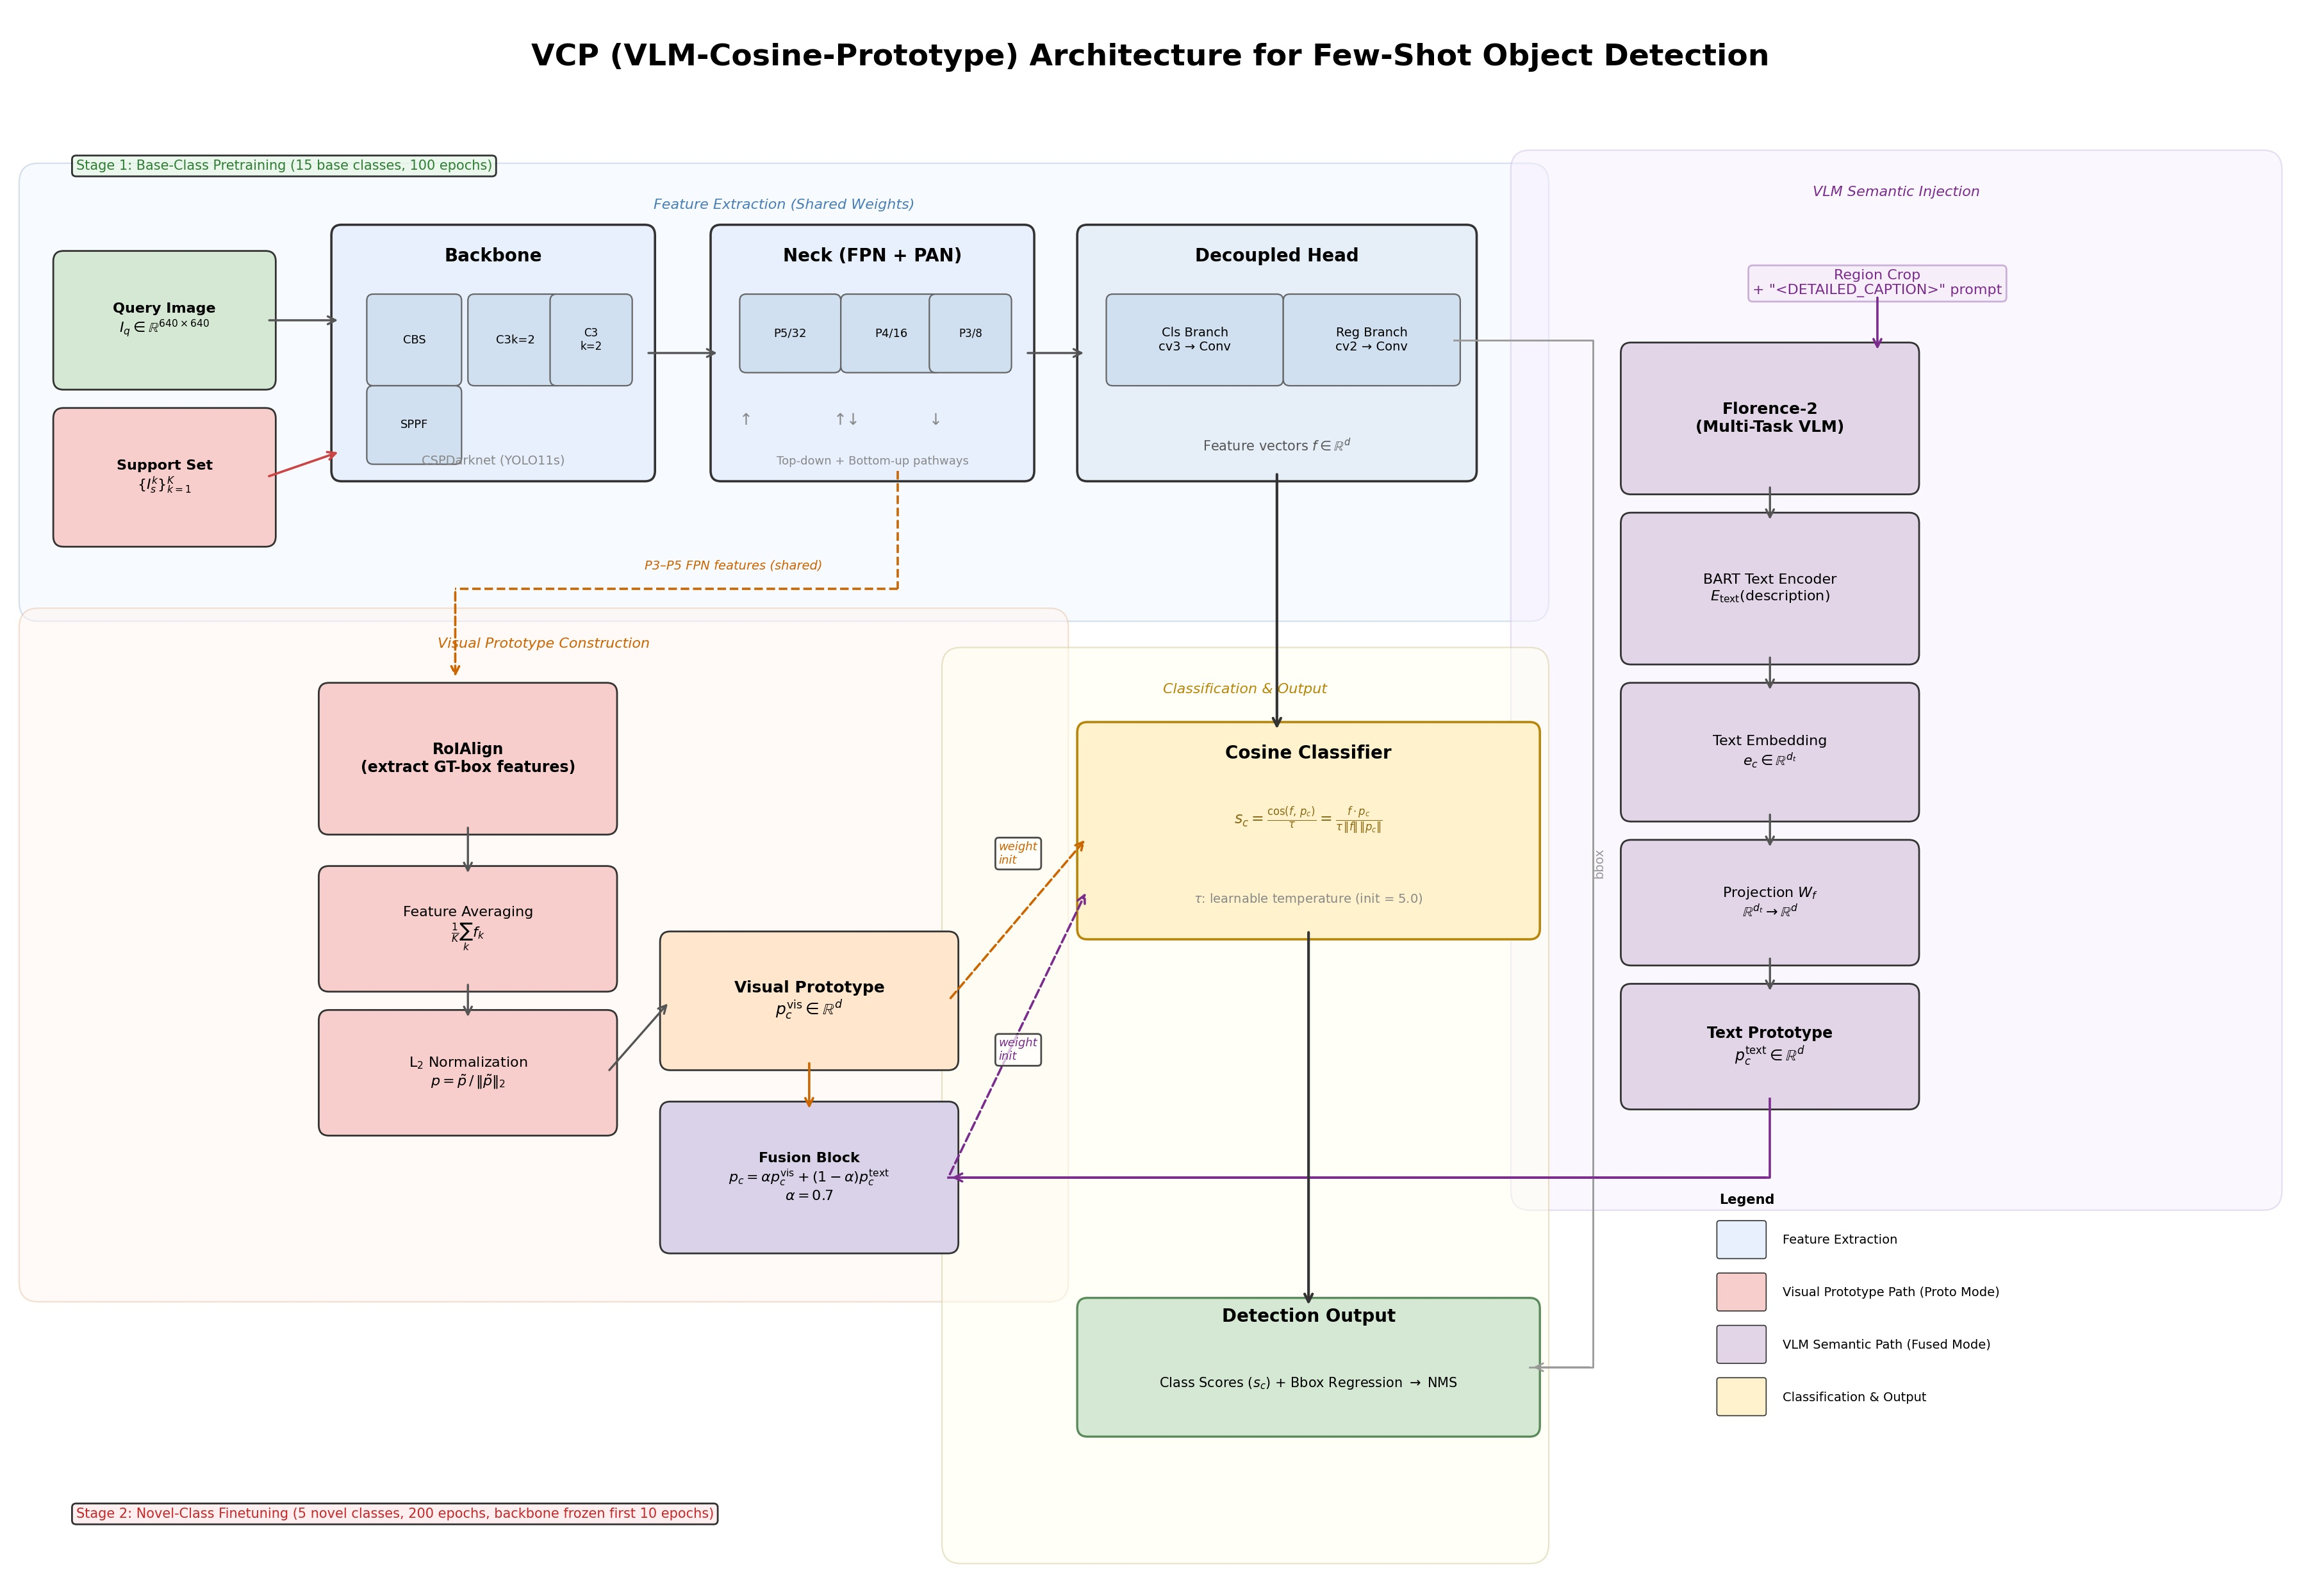
\includegraphics[width=\textwidth]{fig1_framework.jpg}
\caption{VCP framework: YOLO11s backbone+neck $\rightarrow$ decoupled head $\rightarrow$ cosine classifier. Visual prototypes are extracted from support-set via RoIAlign; semantic prototypes from Florence-2 $\rightarrow$ BART encoder. Fused at $\alpha=0.7$.}
\label{fig:framework}
\end{figure*}

Prototypes are constructed from two complementary sources. \textbf{Visual Prototype (Proto mode):} For each novel class $c$ with $K$ support samples, RoIAlign extracts features within ground-truth boxes from FPN levels P3--P5 at the classification branch input (cv3 layer). Averaging and L2-normalizing yields $p_c^{\text{vis}} = \frac{1}{K}\sum_{i=1}^K \text{RoIAlign}(F_i, b_i)$, directly written into the cosine classifier weights.

\textbf{Semantic Prototype \& Fused mode:} Target region crops are fed to Florence-2 with the \texttt{<DETAILED\_CAPTION>} prompt, and the resulting textual descriptions are encoded via BART to produce $p_c^{\text{text}}$. The final prototype fuses both sources with a learnable weight:
\begin{equation}
p_c = \alpha \cdot p_c^{\text{vis}} + (1 - \alpha) \cdot W_f \cdot p_c^{\text{text}}
\label{eq:fused}
\end{equation}
where $\alpha=0.7$ and $W_f$ is a learnable projection matrix. Critically, semantic prototype extraction occurs only during training; at inference, prototypes are fixed in the classifier weights, incurring zero VLM overhead.

\subsection{Cosine Classifier as a Recall Booster}

The gradient of cosine similarity w.r.t.\ feature $f$ reveals the mechanism behind its behavioral pattern:
\begin{equation}
\frac{\partial \cos(f, p_c)}{\partial f} = \frac{p_c - \cos(f, p_c) \cdot f}{\|f\|}
\label{eq:gradient}
\end{equation}
When $f$ has low similarity to $p_c$, the gradient magnitude is large, driving the decision boundary outward. When similarity is already high, gradients diminish. Unlike linear classifiers whose gradient $\partial(W_c f)/\partial f = W_c$ is uniform, the cosine classifier \textit{disproportionately updates low-confidence samples}, naturally favoring a ``better safe than sorry'' strategy: it detects more true positives (high recall) but admits more false positives (low precision). We term this property the \textbf{Recall Booster}. Whether this yields a net mAP gain depends on the product of baseline recall headroom and the dataset's P-R tradeoff ratio, as validated in Section~IV.

\section{Experiments}

\subsection{Setup}

We evaluate on PASCAL VOC 2007+2012 and MS COCO 2014 under the TFA split protocol~\cite{wang2020tfa}: VOC's 20 classes partitioned into 15 base / 5 novel (3 splits); COCO's 20 VOC-overlapping classes as novel, 60 as base. Base detector is YOLO11s (9.5M params), pre-trained on COCO base classes. Stage 1: 100 epochs on base classes, batch 64, lr 0.01. Stage 2: fine-tune on novel classes up to 200 epochs with early stopping (patience 30), batch 4, lr 0.0005. SGD optimizer (momentum 0.937, weight decay 0.0005, 3-epoch warmup), backbone frozen first 10 epochs. Data augmentation: mosaic, RandAugment, random flip, HSV jitter, translation, scaling, and random erasing. Input size $640\times640$. Temperature $\tau$ initialized at 5.0 (learnable). All experiments on a single NVIDIA H20 GPU.

Four variants are compared: (1) \textit{Finetune}---standard YOLO11s with linear classifier; (2) \textit{Cosine}---cosine classifier, random initialization; (3) \textit{Cosine+Proto}---cosine classifier initialized with visual prototypes; (4) \textit{Cosine+Fused}---cosine classifier with visual + Florence-2 fused prototypes.

\subsection{Main Results}

\textbf{VOC Results.} Table~\ref{tab:voc_main} presents VOC mAP50 (Split 1 / 3-split mean $\pm$ std). Three trends emerge: (1) The cosine classifier drives a qualitative leap---5-shot mean: 32.9\% $\rightarrow$ 57.8\% (+24.9 pp); 10-shot: 51.3\% $\rightarrow$ 69.0\% (+17.7 pp). (2) Visual prototype initialization contributes +2.7 pp at 10-shot (mean). (3) Florence-2 fusion adds a consistent +0.5 pp across all three 10-shot splits, limited but directionally positive.

\begin{table*}[t]
\centering\footnotesize
\caption{VOC mAP50 (Split 1 / 3-Split Mean $\pm$ Std)}
\label{tab:voc_main}
\begin{tabular}{lcccc}
\toprule
Method & 1-shot & 3-shot & 5-shot & 10-shot \\
\midrule
Finetune      & 10.9 / --   & 20.5 / --    & 32.9 / --    & 51.3 / --     \\
Cosine        & 12.8 / --   & 51.3 / --    & 66.9 / 57.8$\pm$2.9 & 70.7 / 69.0$\pm$3.1 \\
Cosine+Proto  & 21.5 / --   & 52.3 / --    & 68.8 / 57.8$\pm$2.8 & 74.4 / 71.7$\pm$2.7 \\
Cosine+Fused  & \textbf{21.3} / -- & \textbf{53.9} / -- & \textbf{69.0} / 58.1$\pm$2.5 & \textbf{74.7} / \textbf{72.2}$\pm$2.6 \\
\bottomrule
\end{tabular}
\end{table*}

\textbf{COCO Results.} Table~\ref{tab:coco_main} shows a contrasting pattern: Finetune outperforms all cosine variants. At 30-shot, Cosine+Fused reaches 52.3\%, improving over pure Cosine (49.4\%) but still below Finetune (60.3\%). Results are on a single split and require further verification.

\begin{table}[ht]
\centering
\caption{COCO mAP50}
\label{tab:coco_main}
\begin{tabular}{lcc}
\toprule
Method & 10-shot & 30-shot \\
\midrule
Finetune      & \textbf{59.0} & \textbf{60.3} \\
Cosine        & 47.1 & 49.4 \\
Cosine+Proto  & 47.2 & 51.6 \\
Cosine+Fused  & 47.0 & 52.3 \\
\bottomrule
\end{tabular}
\end{table}

\subsection{P-R Analysis and the P-R Tradeoff Hypothesis}

To explain the VOC-COCO divergence, we decompose Precision and Recall across all 24 method $\times$ shot $\times$ dataset combinations. Table~\ref{tab:pr_summary} summarizes the key patterns.

\begin{table}[ht]
\centering\footnotesize
\caption{P-R Decomposition Summary}
\label{tab:pr_summary}
\begin{tabular}{lcccc}
\toprule
Setting & $\Delta$P & $\Delta$R & $\Delta$mAP & $\Delta$R/$|\Delta$P$|$ \\
\midrule
VOC 5-shot Cos+Fused & $-$0.22 & +0.45 & +35.9 & 2.00 \\
VOC 10-shot Cos+Fused& $-$0.35 & +0.33 & +23.4 & 0.96 \\
COCO 10-shot Cos+Fused&$-$0.81& +0.39 & $-$12.0 & 0.48 \\
COCO 30-shot Cos+Fused&$-$0.56& +0.14 & $-$8.0 & 0.25 \\
\bottomrule
\end{tabular}
\end{table}

Three findings emerge from the full decomposition (all changes relative to Finetune baseline):

\textbf{Finding 1---Invariant Recall Booster Behavior:} Across all 24 comparisons, every cosine variant \textit{without exception} shifts the operating point toward higher recall and lower precision. The directionality is perfectly consistent---this is a systematic property, not a conditional artifact (see gradient analysis, Section~III-B).

\textbf{Finding 2---Tradeoff Ratio Determines Net Benefit:} On VOC, each unit of recall gain costs relatively little precision ($\Delta$R/$|\Delta$P$| \approx 2.0$ at 5-shot), and the large recall boost dominates. On COCO, the ratio collapses: $\Delta$R/$|\Delta$P$| \approx 0.48$ at 10-shot and 0.25 at 30-shot, as precision plummets from 0.895 to 0.084. COCO's 20 novel classes (vs.\ 5 on VOC) and higher scene complexity cause the cosine classifier's relaxed decision boundary to generate massive cross-class false positives.

\textbf{Finding 3---Fused Mode Modulates P-R Balance:} At VOC 10-shot, Fused (P=0.200, R=0.872) vs.\ pure Cosine (P=0.336, R=0.848) partially recovers precision (+0.136) with minimal recall loss ($-$0.024), suggesting semantic priors help moderate the over-relaxation of visual prototypes.

We formalize these observations as the \textbf{P-R Tradeoff Hypothesis}:

\begin{quote}\small
The cosine classifier inherently pushes the detector toward a high-recall, low-precision operating point. Net benefit is determined by the product of: (1) baseline recall headroom, and (2) the dataset's P-R tradeoff ratio (driven by class count and scene complexity). VOC possesses both low baseline recall and a favorable tradeoff ratio, yielding significant gains; COCO faces an unfavorable tradeoff ratio, where precision loss dominates.
\end{quote}

\begin{figure*}[t]
\centering
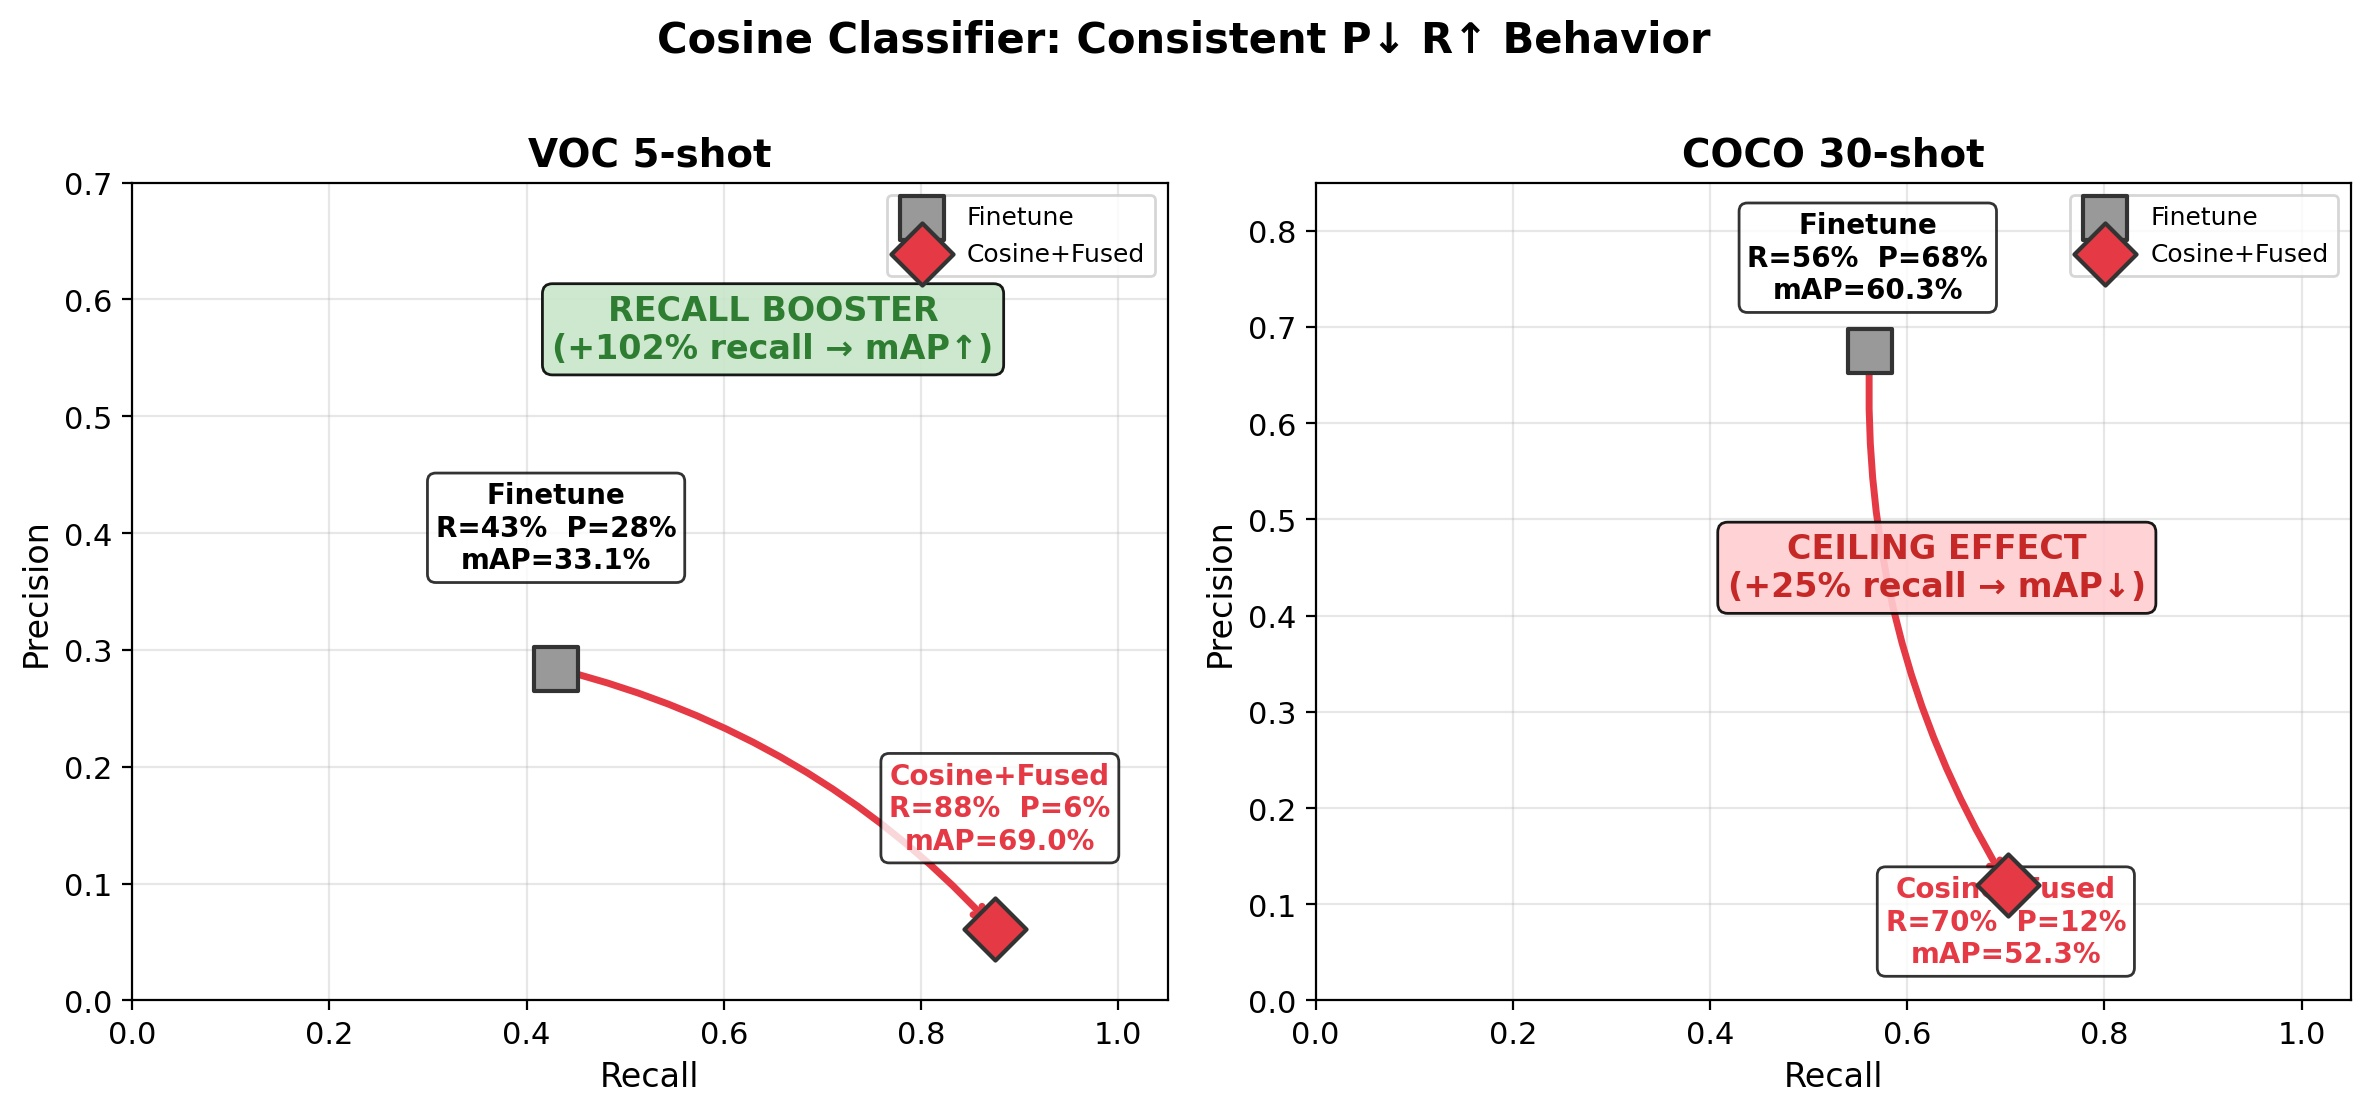
\includegraphics[width=\textwidth]{fig3_pr_comparison.jpg}
\caption{VOC 5-shot vs.\ COCO 30-shot Precision-Recall comparison, validating the P-R Tradeoff Hypothesis.}
\label{fig:pr_comparison}
\end{figure*}

\subsection{Ablation and SOTA Comparison}

\textbf{Ablation.} Table~\ref{tab:ablation} merges component and prototype source ablations. The cosine head is the dominant driver ($\sim$90\% of gains). Visual prototypes alone (74.4\%) outperform Florence-2 text-only (72.1\%), and fusion achieves the optimum (74.7\%), confirming complementary value.

\begin{table}[ht]
\centering\footnotesize
\caption{Ablation: Component \& Prototype Source (VOC)}
\label{tab:ablation}
\begin{tabular}{lrrr}
\toprule
Configuration & 3-shot & 5-shot & 10-shot \\
\midrule
Finetune (baseline) & 20.5 & 32.9 & 51.3 \\
~~+ Cosine head    & 51.3 & 66.9 & 70.7 \\
~~+ Visual Proto   & 52.3 & 68.8 & 74.4 \\
~~+ VLM Fused      & 53.9 & 69.0 & \textbf{74.7} \\
Florence-2 Only (10-shot) & --- & --- & 72.1 \\
\bottomrule
\end{tabular}
\end{table}

\textbf{SOTA Comparison.} Table~\ref{tab:sota} compares VCP against existing FSOD methods (VOC Split 1). All baselines use Faster R-CNN R-101 ($\sim$60M), VCP uses YOLO11s ($\sim$9.5M). At 5-shot and 10-shot, VCP matches or surpasses all prior methods while using $\sim$1/6 the parameters. The 1-shot gap indicates single-stage detectors need additional regularization under extreme scarcity.

\begin{table}[ht]
\centering\footnotesize
\caption{Comparison with SOTA (VOC Split 1, mAP50)}
\label{tab:sota}
\begin{tabular}{lcccc}
\toprule
Method & 1-shot & 3-shot & 5-shot & 10-shot \\
\midrule
TFA w/cos        & 39.8 & 44.7 & 55.7 & 56.0 \\
FSCE             & 44.2 & 51.4 & 61.9 & 63.4 \\
DeFRCN           & 53.6 & 61.5 & 64.1 & 60.8 \\
KD-DeFRCN        & \textbf{58.2} & \textbf{65.1} & 68.2 & 67.4 \\
\midrule
VCP Cos+Fused    & 21.3 & 53.9 & \textbf{69.0} & \textbf{74.7} \\
VCP Cos+Proto    & 21.5 & 52.3 & 68.8 & 74.4 \\
\bottomrule
\end{tabular}
\end{table}

\subsection{Inference Speed}

Table~\ref{tab:fps} compares inference speed (NVIDIA H20, $640\times640$, batch 1). VCP Fused achieves 54.4 FPS---4--5$\times$ faster than two-stage FSOD methods---with only 9.4M parameters. The cosine classifier adds $\sim$4 ms latency (from L2 normalization), still well above the 30 FPS real-time threshold. Critically, Florence-2 is \textit{not} loaded at inference; semantic prototypes are pre-computed and stored in the classifier weights.

\begin{table}[ht]
\centering
\caption{Inference Speed (H20, $640\times640$, bs=1)}
\label{tab:fps}
\begin{tabular}{lccc}
\toprule
Model & Latency (ms) & FPS & Params \\
\midrule
FRCN R-101 (ref.) & $\sim$85 & $\sim$12 & $\sim$60M \\
\midrule
YOLO11s baseline & 14.4 & 69.5 & 9.4M \\
Finetune          & 14.7 & 68.2 & 9.4M \\
Cosine            & 18.9 & 52.8 & 9.4M \\
Fused (VCP)       & 18.4 & \textbf{54.4} & 9.4M \\
\bottomrule
\end{tabular}
\end{table}

\section{Conclusion}

We presented VCP, a single-stage FSOD framework integrating YOLO11s with cosine classification and prototype learning. Key findings: (1) Single-stage FSOD is viable---VCP achieves competitive performance at 1/6 the parameter count of two-stage methods, with 54.4 FPS real-time inference. (2) Through 24-group P-R decomposition, we identified the cosine classifier's Recall Booster property and formulated the P-R Tradeoff Hypothesis explaining VOC-COCO divergence via the product of baseline recall headroom and dataset tradeoff ratio. (3) Florence-2 semantic prototypes provide directionally consistent but limited gains (+0.5 pp at 10-shot), with zero inference overhead.

Limitations include weak 1-shot performance, single-split COCO evaluation, and the post-hoc nature of the tradeoff hypothesis. Future work will explore adaptive VLM fusion, cross-domain FSOD generalization, and independent validation of the hypothesis on additional datasets.

\begin{thebibliography}{99}

\bibitem{sun2021fsce}
B.~Sun et al., ``FSCE: Few-shot object detection via contrastive proposal encoding,'' in \emph{CVPR}, 2021, pp. 7352--7362.

\bibitem{qiao2021defrcn}
L.~Qiao et al., ``DeFRCN: Decoupled faster R-CNN for few-shot object detection,'' in \emph{ICCV}, 2021, pp. 8681--8690.

\bibitem{ren2015faster}
S.~Ren et al., ``Faster R-CNN: Towards real-time object detection with region proposal networks,'' in \emph{NeurIPS}, 2015.

\bibitem{redmon2016yolo}
J.~Redmon et al., ``You only look once: Unified, real-time object detection,'' in \emph{CVPR}, 2016, pp. 779--788.

\bibitem{jocher2023ultralytics}
G.~Jocher et al., ``Ultralytics YOLO (version 8.0),'' 2023. [Online]. Available: \url{https://github.com/ultralytics/ultralytics}

\bibitem{wang2020tfa}
X.~Wang et al., ``Frustratingly simple few-shot object detection,'' in \emph{ICML}, 2020, pp. 9919--9928.

\bibitem{radford2021clip}
A.~Radford et al., ``Learning transferable visual models from natural language supervision,'' in \emph{ICML}, 2021, pp. 8748--8763.

\bibitem{xiao2024florence2}
B.~Xiao et al., ``Florence-2: Advancing a unified representation for a variety of vision tasks,'' in \emph{CVPR}, 2024, pp. 4818--4829.

\bibitem{yan2019meta}
X.~Yan et al., ``Meta R-CNN: Towards general solver for instance-level low-shot learning,'' in \emph{ICCV}, 2019, pp. 9577--9586.

\bibitem{wang2019meta}
Y.-X.~Wang et al., ``Meta-learning to detect rare objects,'' in \emph{ICCV}, 2019, pp. 9925--9934.

\bibitem{pei2022kddefrcn}
W.~Pei et al., ``Few-shot object detection by knowledge distillation using bag-of-visual-words representations,'' in \emph{ECCV}, 2022, pp. 283--300.

\bibitem{wu2020mpsr}
J.~Wu et al., ``Multi-scale positive sample refinement for few-shot object detection,'' in \emph{ECCV}, 2020, pp. 456--472.

\bibitem{xiao2020fsdetview}
Y.~Xiao and R.~Marlet, ``Few-shot object detection and viewpoint estimation for objects in the wild,'' in \emph{ECCV}, 2020, pp. 192--210.

\bibitem{li2021cme}
B.~Li et al., ``Beyond max-margin: Class margin equilibrium for few-shot object detection,'' in \emph{CVPR}, 2021, pp. 7363--7372.

\bibitem{redmon2018yolov3}
J.~Redmon and A.~Farhadi, ``YOLOv3: An incremental improvement,'' arXiv:1804.02767, 2018.

\bibitem{kang2019fsrw}
B.~Kang et al., ``Few-shot object detection via feature reweighting,'' in \emph{ICCV}, 2019, pp. 8420--8429.

\bibitem{minderer2022owlvit}
M.~Minderer et al., ``Simple open-vocabulary object detection with vision transformers,'' in \emph{ECCV}, 2022.

\bibitem{li2022glip}
L.~H.~Li et al., ``Grounded language-image pre-training,'' in \emph{CVPR}, 2022, pp. 10965--10975.

\bibitem{liu2023groundingdino}
S.~Liu et al., ``Grounding DINO: Marrying DINO with grounded pre-training for open-set object detection,'' arXiv:2303.05499, 2023.

\end{thebibliography}

\end{document}
